\chapter{Stereokimia: Kiralitas dan Isomer}\label{ch:g12:stereochemistry}

Daun mint hijau dan biji jintan Belanda baunya sama sekali tidak mirip:
yang satu berbau segar seperti permen karet, yang lain berbau hangat
seperti roti gandum hitam. Padahal \omterm{def:g7:atoms-and-molecules:molecule}{molekul} yang menimbulkan kedua bau
itu sama-sama karvon, yang tersusun atas \omterm{def:g7:atoms-and-molecules:atom}{atom-atom} yang sama, terikat
dalam urutan yang sama. Kedua karvon itu hanya berbeda seperti tangan
kiri berbeda dari tangan kanan: yang satu adalah bayangan cermin yang
lain. Hidung kita, yang tersusun atas \omterm{def:g7:atoms-and-molecules:molecule}{molekul-molekul} yang juga
``bertangan'', dapat membedakan keduanya. Bab ini belajar melihat
\omterm{def:g7:atoms-and-molecules:molecule}{molekul} dalam tiga dimensi.

\begin{recall}
Bentuk \omterm{def:g7:atoms-and-molecules:molecule}{molekul}, serta baji yang menggambarkannya di dalam ruang
(\cref{ch:g10:lewis-and-shape}). \omterm{def:g11:organic-skeletons:isomer}{Isomer struktur}
(\cref{ch:g11:organic-skeletons}). \omterm{def:g11:functional-groups:functional-group}{Gugus fungsi}
(\cref{ch:g11:functional-groups}).
\end{recall}

\begin{omfigure}
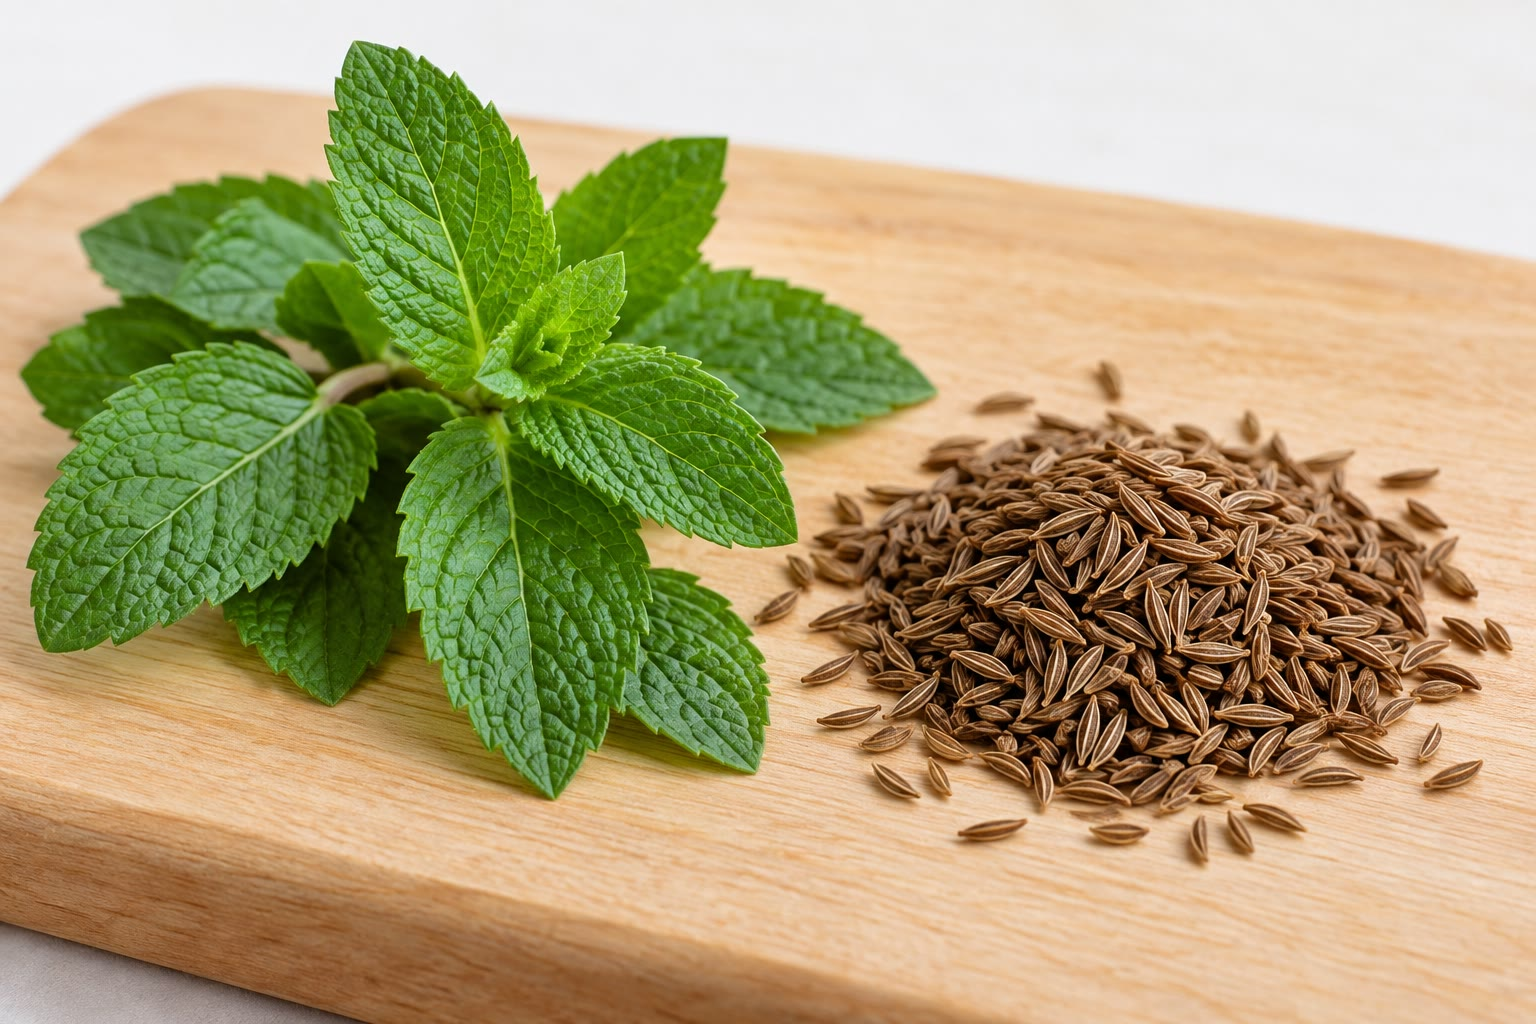
\includegraphics[width=0.48\linewidth]{images/book1/ai/g12-mint-caraway.jpg}

{\small Mint hijau dan jintan Belanda: dua \omterm{def:g7:atoms-and-molecules:molecule}{molekul} yang saling bayangan
cermin, dua bau.}
\end{omfigure}

\section{Molekul di dalam ruang}

\begin{definition}[Stereoisomer]\label{def:g12:stereochemistry:stereoisomer}
Yang disebut \emph{stereoisomer}\index{stereoisomer} adalah
\omterm{def:g7:atoms-and-molecules:molecule}{molekul-molekul} dengan rumus yang sama dan urutan \omterm{def:g7:atoms-and-molecules:atom}{atom} terikat yang
sama, yang hanya berbeda dalam susunan \omterm{def:g7:atoms-and-molecules:atom}{atom-atomnya} di dalam ruang.
\end{definition}

\begin{definition}[Representasi Cram]\label{def:g12:stereochemistry:cram}
Dalam \emph{representasi Cram}\index{representasi Cram} sebuah \omterm{def:g7:atoms-and-molecules:atom}{atom}
karbon dengan empat ikatan tunggal, dua ikatan digambar pada bidang
kertas sebagai garis biasa, membentuk sudut, ikatan yang mengarah ke
pembaca sebagai baji pejal, dan ikatan yang mengarah menjauh sebagai
baji putus-putus.
\end{definition}

\section{Kiralitas}

\begin{definition}[Kiral, karbon asimetris]\label{def:g12:stereochemistry:chiral}
Sebuah benda atau \omterm{def:g7:atoms-and-molecules:molecule}{molekul} disebut \emph{kiral}\index{kiral} jika tidak
dapat ditumpangtindihkan dengan bayangan cerminnya, seperti tangan.
\omterm{def:g7:atoms-and-molecules:atom}{Atom} karbon yang terikat pada empat \omterm{def:g7:atoms-and-molecules:atom}{atom} atau gugus yang berbeda
disebut \emph{karbon asimetris}\index{karbon asimetris}; karbon itu
sering ditandai dengan bintang.
\end{definition}

\begin{proposition}[Satu karbon asimetris membuat molekul kiral]\label{prop:g12:stereochemistry:one-carbon}
\omterm{def:g7:atoms-and-molecules:molecule}{Molekul} dengan tepat satu \omterm{def:g12:stereochemistry:chiral}{karbon asimetris} bersifat \omterm{def:g12:stereochemistry:chiral}{kiral}.
\end{proposition}

\begin{proof}
Diterima tanpa bukti: menukar dua dari keempat gugus berbeda di sekitar
\omterm{def:g12:stereochemistry:chiral}{karbon asimetris} menghasilkan bayangan cerminnya, dan tidak ada rotasi
seluruh \omterm{def:g7:atoms-and-molecules:molecule}{molekul} yang dapat mengembalikannya, karena keempat gugus itu
semuanya berbeda.
\end{proof}

\begin{definition}[Enantiomer, campuran rasemat]\label{def:g12:stereochemistry:enantiomer}
Dua \omterm{def:g12:stereochemistry:stereoisomer}{stereoisomer} yang saling bayangan cermin dan tidak dapat
ditumpangtindihkan disebut \emph{enantiomer}\index{enantiomer}.
\omterm{def:g6:pure-substances-and-mixtures:mixture}{Campuran} dua enantiomer dalam jumlah yang sama disebut
\emph{campuran rasemat}\index{campuran rasemat}.
\end{definition}

\begin{omfigure}
\setchemfig{atom sep=2.2em}
\begin{tikzpicture}[font=\small]
  \node at (-2.4,0) {\chemfig{C(-[2]COOH)(-[4]H_3C)(<[:-30]OH)(<:[:-150]H)}};
  \node at (2.4,0) {\chemfig{C(-[2]COOH)(-[0]CH_3)(<[:-150]HO)(<:[:-30]H)}};
  \draw[dashed, omDef, thick] (0,-1.5) -- (0,1.6) node[above] {cermin};
  \node[anchor=north] at (-2.4,-1.4) {asam laktat, A};
  \node[anchor=north] at (2.4,-1.4) {bayangan cerminnya, B};
\end{tikzpicture}

{\small Kedua \omterm{def:g12:stereochemistry:enantiomer}{enantiomer} asam laktat, \ce{CH3-CH(OH)-COOH}, dalam
\omterm{def:g12:stereochemistry:cram}{representasi Cram}. Karbon pusatnya asimetris (\ce{H}, \ce{OH},
\ce{CH3}, \ce{COOH}). Tidak ada rotasi yang mengubah A menjadi B:
keduanya berbeda seperti tangan kiri dan tangan kanan.}
\end{omfigure}

\begin{method}[Apakah sebuah molekul kiral?]\label{met:g12:stereochemistry:chiral}
\begin{enumerate}
  \item Carilah \omterm{def:g12:stereochemistry:chiral}{karbon asimetris}: karbon dengan empat gugus yang
        berbeda. Tidak ada: \omterm{def:g7:atoms-and-molecules:molecule}{molekul} itu (dalam buku ini) tidak \omterm{def:g12:stereochemistry:chiral}{kiral}.
  \item Tepat satu: \omterm{def:g7:atoms-and-molecules:molecule}{molekul} itu \omterm{def:g12:stereochemistry:chiral}{kiral}.
  \item Dua atau lebih: carilah bidang yang membelah \omterm{def:g7:atoms-and-molecules:molecule}{molekul} menjadi dua
        belahan yang saling bayangan cermin, dalam salah satu bentuknya;
        jika bidang itu ada, \omterm{def:g7:atoms-and-molecules:molecule}{molekulnya} tidak \omterm{def:g12:stereochemistry:chiral}{kiral}, jika tidak ada,
        \omterm{def:g7:atoms-and-molecules:molecule}{molekulnya} \omterm{def:g12:stereochemistry:chiral}{kiral}.
\end{enumerate}
\end{method}

\begin{remark}[Sifat sama, bau berbeda]\label{rem:g12:stereochemistry:same}
% ledger: smell:carvone-R, smell:carvone-S
Dua \omterm{def:g12:stereochemistry:enantiomer}{enantiomer} memiliki suhu leleh dan suhu didih yang sama, \omterm{def:g6:solutions-and-solubility:solubility}{kelarutan}
yang sama, spektrum yang sama: setiap pengukuran yang dilakukan dengan
sesuatu yang tidak \omterm{def:g12:stereochemistry:chiral}{kiral} memberikan hasil yang sama bagi keduanya.
Keduanya hanya berbeda ketika bertemu dengan sesuatu yang \omterm{def:g12:stereochemistry:chiral}{kiral}, seperti
cahaya terpolarisasi, yang diputar keduanya ke arah berlawanan, atau
reseptor di hidung: karvon yang satu berbau mint hijau, \omterm{def:g12:stereochemistry:enantiomer}{enantiomernya}
berbau jintan Belanda.
\end{remark}

\section{Diastereomer}

\begin{definition}[Diastereomer]\label{def:g12:stereochemistry:diastereomer}
\omterm{def:g12:stereochemistry:stereoisomer}{Stereoisomer} yang tidak saling bayangan cermin disebut
\emph{diastereomer}\index{diastereomer}. Berbeda dengan \omterm{def:g12:stereochemistry:enantiomer}{enantiomer},
diastereomer memiliki sifat fisika yang berbeda.
\end{definition}

\begin{proposition}[Menghitung stereoisomer]\label{prop:g12:stereochemistry:count}
\omterm{def:g7:atoms-and-molecules:molecule}{Molekul} dengan $n$ \omterm{def:g12:stereochemistry:chiral}{karbon asimetris} memiliki paling banyak $2^n$
\omterm{def:g12:stereochemistry:stereoisomer}{stereoisomer}. Jumlahnya lebih sedikit jika \omterm{def:g7:atoms-and-molecules:molecule}{molekul} itu memiliki dua
belahan yang serupa: salah satu kombinasinya lalu memiliki bidang
cermin dan tidak \omterm{def:g12:stereochemistry:chiral}{kiral} (bentuk \emph{meso}).
\end{proposition}

\begin{proof}
Setiap \omterm{def:g12:stereochemistry:chiral}{karbon asimetris} dapat mengambil dua susunan, tidak bergantung
pada karbon lainnya: $2 \times 2 \times \dots \times 2 = 2^n$ kombinasi.
Jika dua kombinasi merupakan \omterm{def:g7:atoms-and-molecules:molecule}{molekul} yang sama, jumlahnya berkurang.
\end{proof}

\begin{omfigure}
\setchemfig{atom sep=1.9em}
\begin{tabular}{ccc}
\chemfig{HOOC-[:-30]C(<[:-90]OH)-[:30]C(<[:90]OH)-[:-30]COOH} &
\chemfig{HOOC-[:-30]C(<:[:-90]OH)-[:30]C(<:[:90]OH)-[:-30]COOH} &
\chemfig{HOOC-[:-30]C(<[:-90]OH)-[:30]C(<:[:90]OH)-[:-30]COOH} \\[4pt]
\small asam L-tartrat & \small asam D-tartrat & \small asam meso-tartrat \\
\small (\omterm{def:g12:stereochemistry:chiral}{kiral}) & \small (\omterm{def:g12:stereochemistry:chiral}{kiral}, bayangan cermin L) & \small (tidak \omterm{def:g12:stereochemistry:chiral}{kiral})
\end{tabular}

{\small Ketiga \omterm{def:g12:stereochemistry:stereoisomer}{stereoisomer} asam tartrat. L dan D adalah \omterm{def:g12:stereochemistry:enantiomer}{enantiomer};
masing-masing merupakan \omterm{def:g12:stereochemistry:diastereomer}{diastereomer} bentuk meso, yang memiliki bidang
cermin dalam salah satu bentuknya: tiga \omterm{def:g12:stereochemistry:stereoisomer}{stereoisomer}, bukan $2^2 = 4$.}
\end{omfigure}

\begin{history}[Pasteur memilah kristal dengan tangan, 1848]
Pada tahun 1848, ahli kimia muda Louis Pasteur mengamati dengan kaca
pembesar kristal-kristal sebuah garam ``asam rasemat'', suatu bentuk
asam tartrat yang tidak memutar cahaya terpolarisasi ke arah mana pun.
Ia memperhatikan bahwa kristal-kristal itu terdapat dalam dua bentuk
yang saling bayangan cermin, dan ia memilahnya satu per satu dengan
pinset. Setelah dilarutkan, tumpukan yang satu memutar cahaya
terpolarisasi ke kanan, yang lain ke kiri dengan besar yang sama: asam
rasemat ternyata \omterm{def:g6:pure-substances-and-mixtures:mixture}{campuran} dua \omterm{def:g7:atoms-and-molecules:molecule}{molekul} yang saling bayangan cermin.
\omterm{def:g7:atoms-and-molecules:molecule}{Molekul}, simpulnya, dapat bertangan.
\end{history}

\begin{omfigure}
\begin{minipage}[t]{0.36\linewidth}\centering
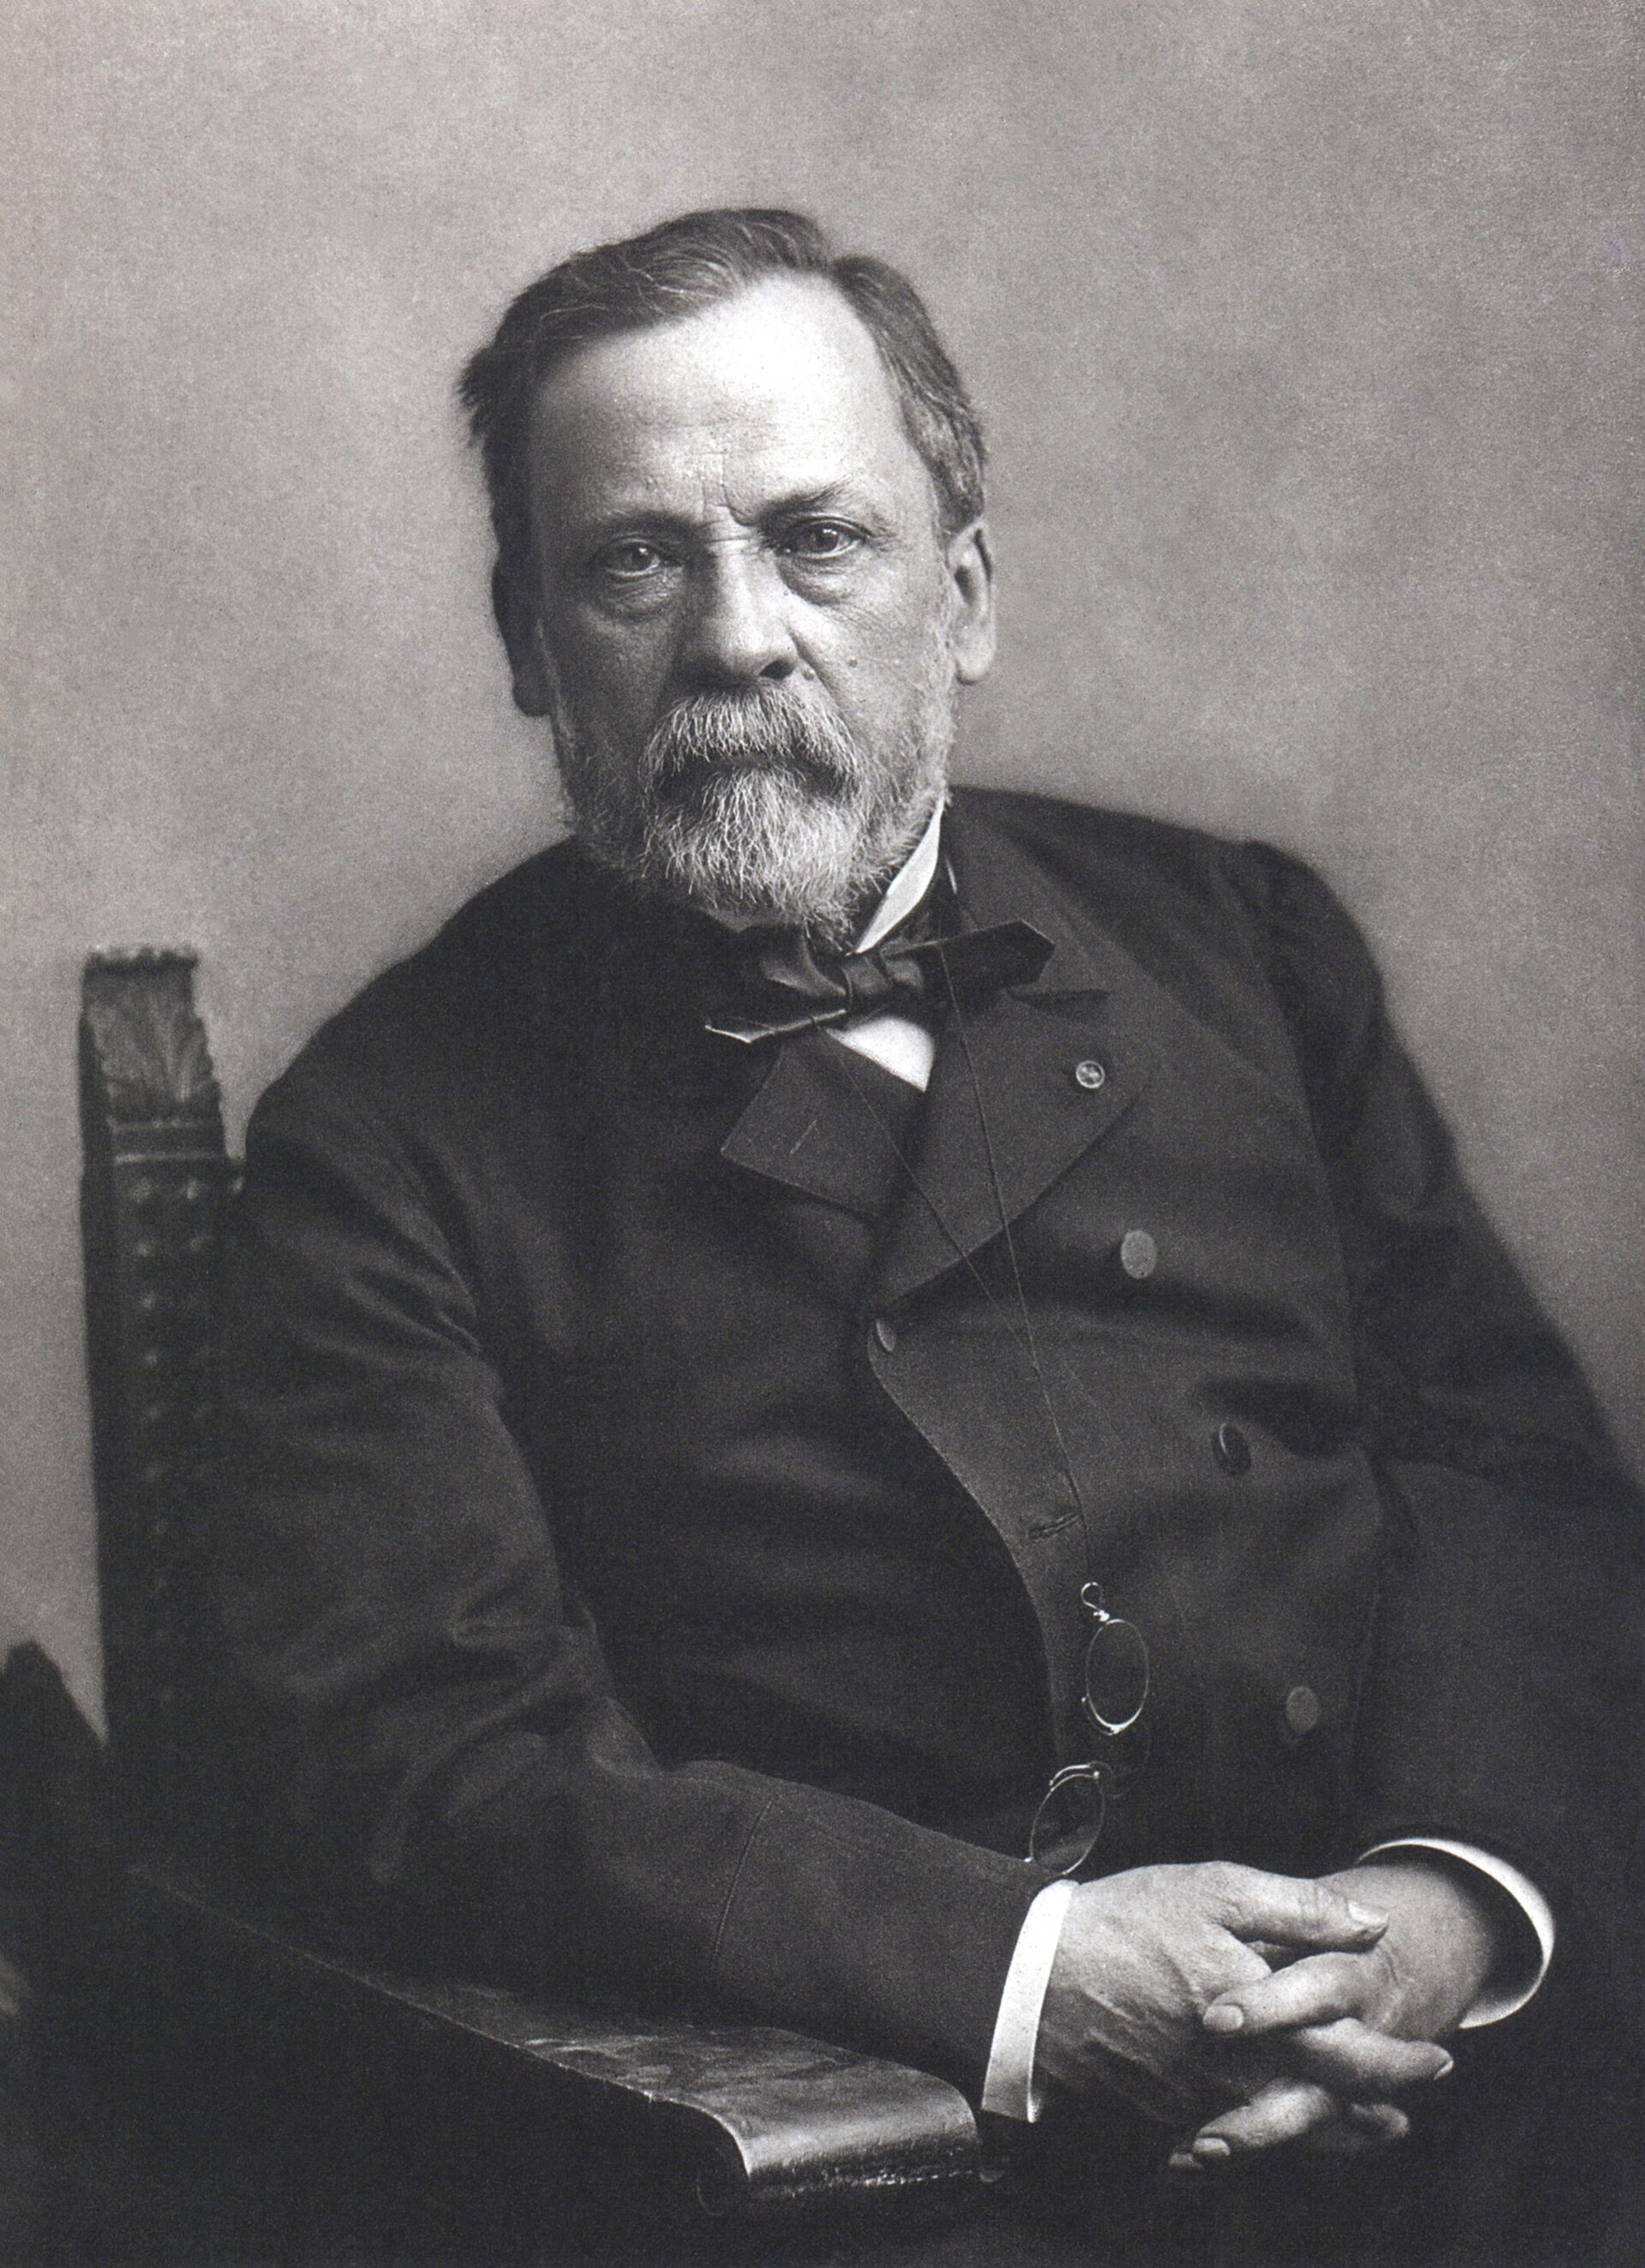
\includegraphics[height=5cm]{images/book1/pasteur.jpg}

{\small Louis Pasteur (1822--1895), dipotret oleh Paul Nadar.}
\end{minipage}\qquad
\begin{minipage}[t]{0.36\linewidth}\centering
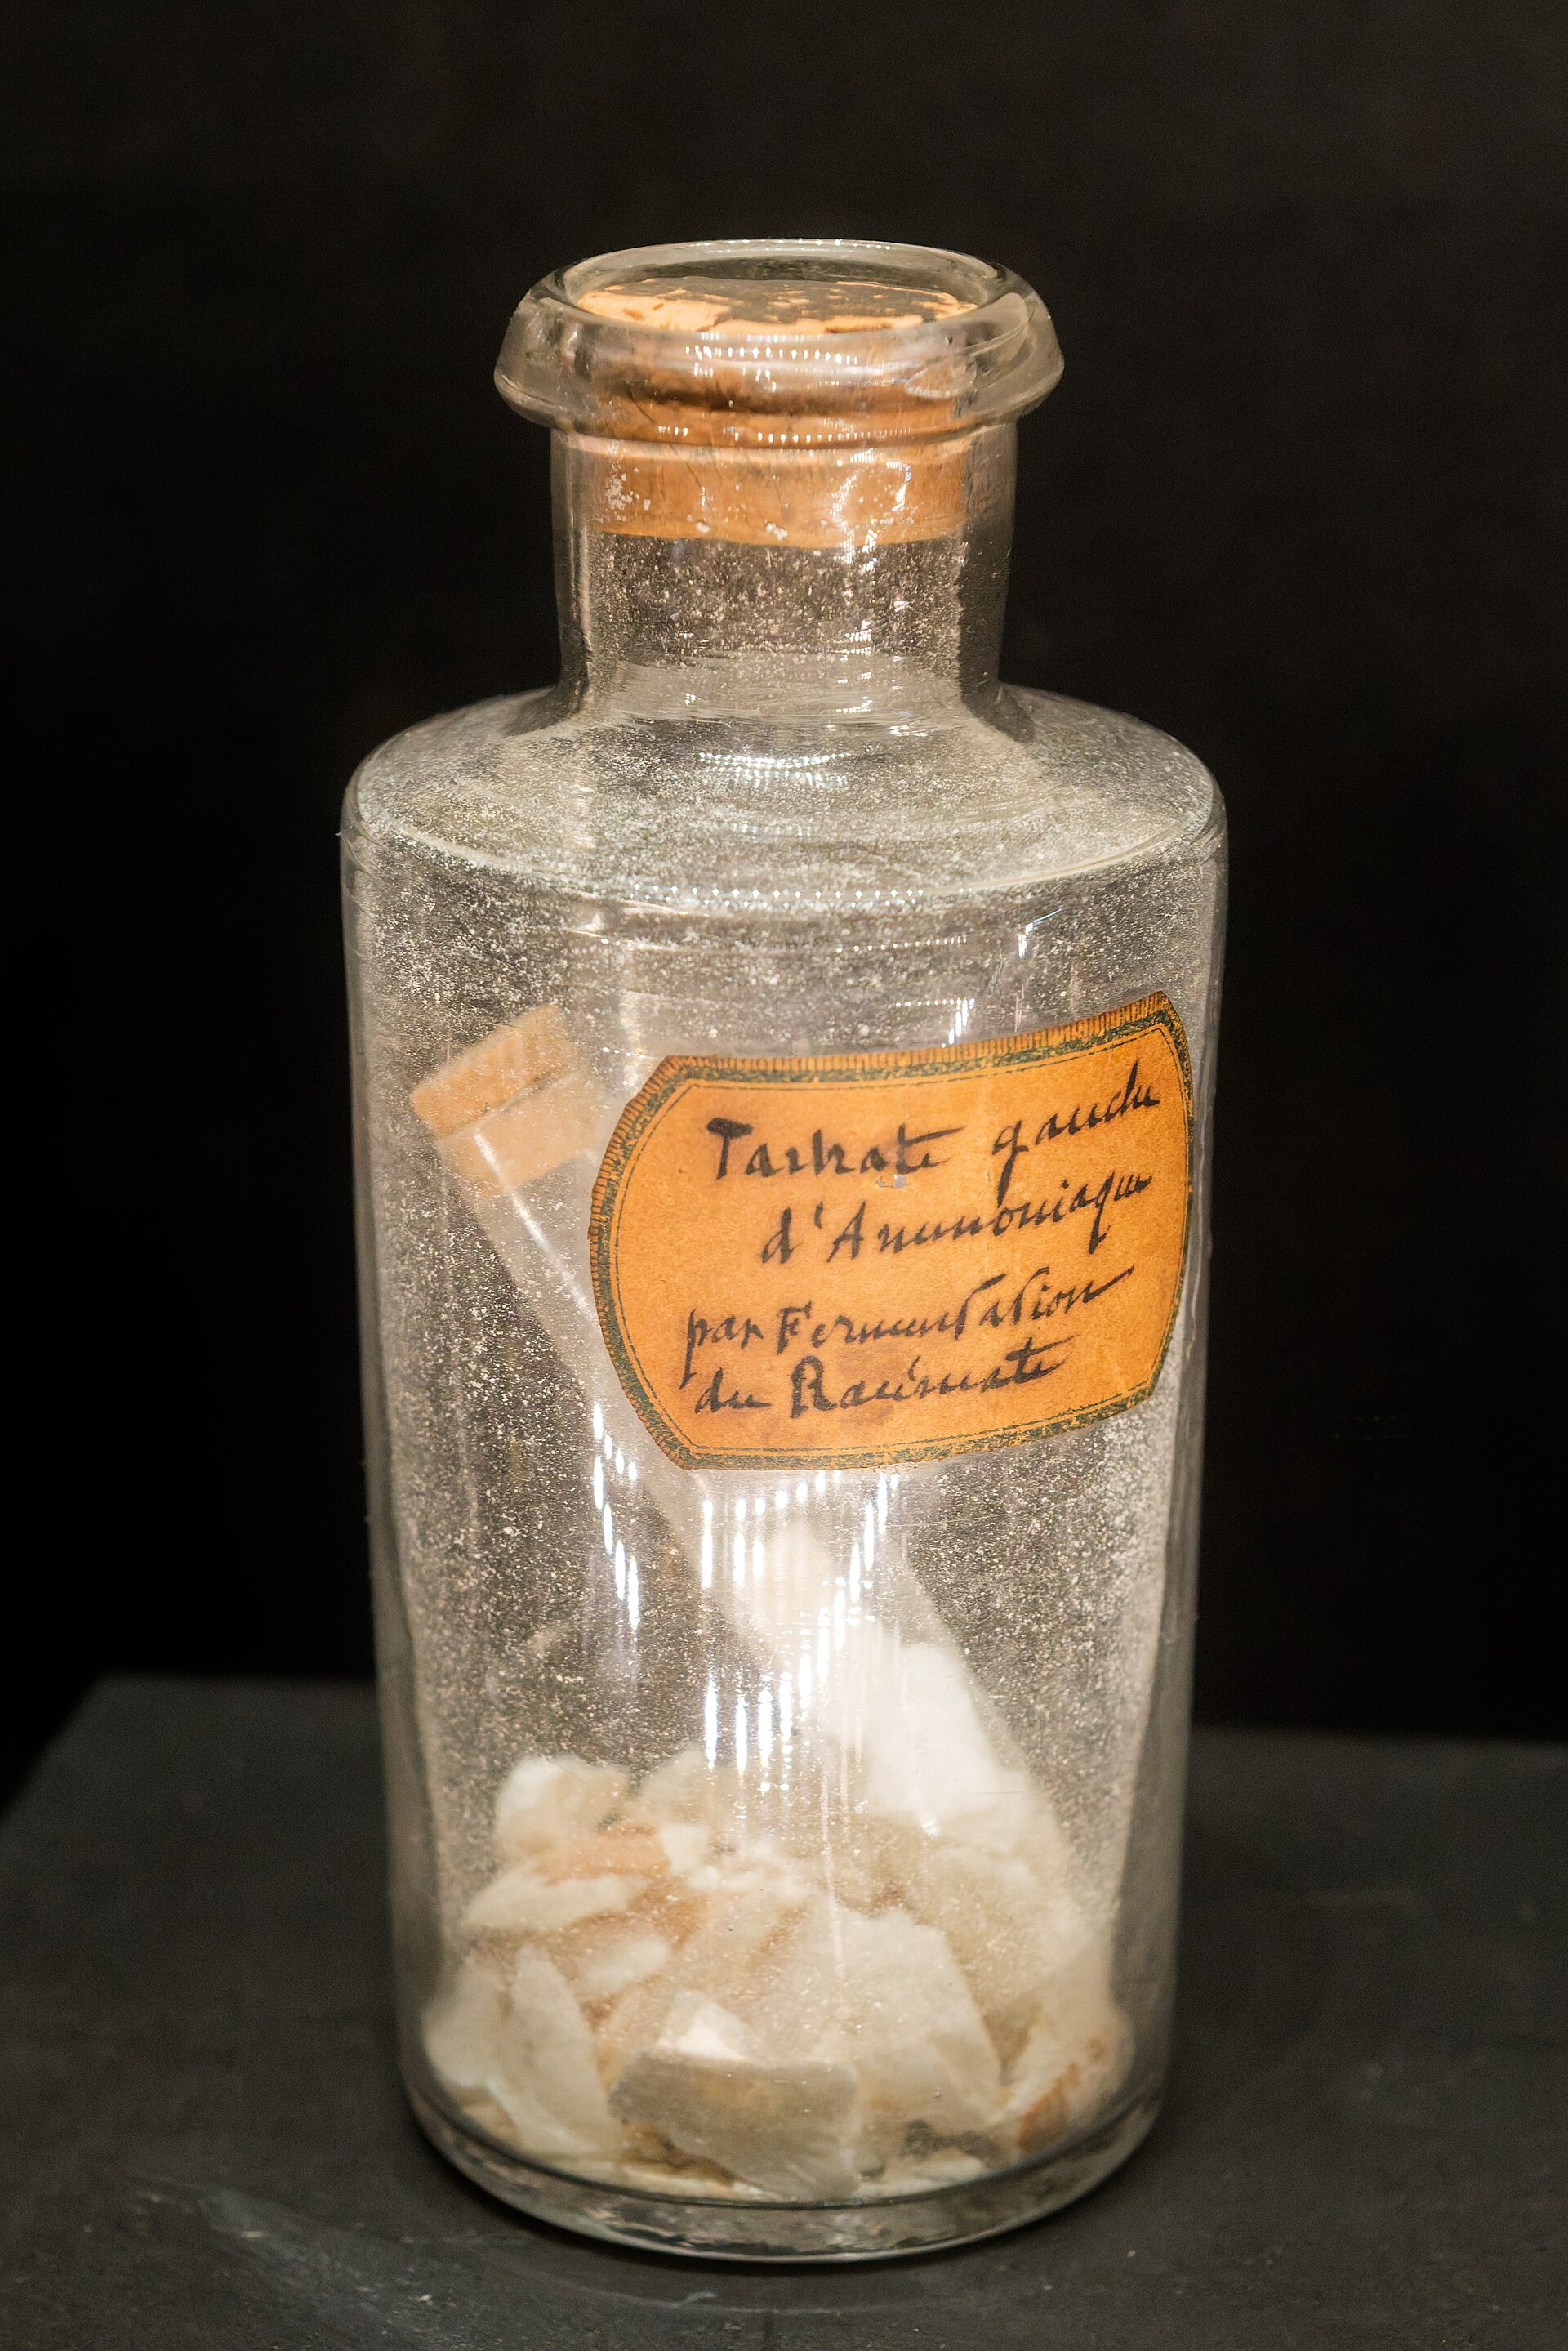
\includegraphics[height=5cm]{images/book1/tartrate-crystals.jpg}

{\small Kristal amonium tartrat dari koleksi Pasteur. Foto: Marie-Lan
Taÿ Pamart, CC\ BY\ 4.0.}
\end{minipage}
\end{omfigure}

\section{Isomer Z dan E}


\begin{definition}[Isomer Z dan E]\label{def:g12:stereochemistry:z-e}
Jika setiap karbon sebuah \omterm{def:g10:lewis-and-shape:multiple-bond}{ikatan rangkap} \ce{C=C} membawa dua \omterm{def:g7:atoms-and-molecules:atom}{atom} atau
gugus yang berbeda, ada dua \omterm{def:g12:stereochemistry:stereoisomer}{stereoisomer}, karena \omterm{def:g10:lewis-and-shape:multiple-bond}{ikatan rangkap} tidak
dapat berotasi. Pada setiap karbon, gugus yang \omterm{def:g7:atoms-and-molecules:atom}{atomnya} terikat langsung
pada karbon itu memiliki \omterm{def:g9:inside-the-atom:atomic-number}{nomor atom} lebih besar mendapat prioritas. Jika
kedua gugus prioritas berada pada sisi yang sama dari \omterm{def:g10:lewis-and-shape:multiple-bond}{ikatan rangkap},
\omterm{def:g11:organic-skeletons:isomer}{isomernya} disebut \emph{Z}\index{isomer Z}; jika keduanya berada pada
sisi yang berlawanan, \omterm{def:g11:organic-skeletons:isomer}{isomernya} disebut \emph{E}\index{isomer E}.
\end{definition}

\begin{method}[Z atau E?]\label{met:g12:stereochemistry:z-e}
\begin{enumerate}
  \item Periksalah bahwa setiap karbon \omterm{def:g10:lewis-and-shape:multiple-bond}{ikatan rangkap} membawa dua gugus
        yang berbeda; jika tidak, tidak ada isomeri \omterm{def:g12:stereochemistry:z-e}{Z}/\omterm{def:g12:stereochemistry:z-e}{E}.
  \item Pada setiap karbon, berikan prioritas kepada gugus yang \omterm{def:g7:atoms-and-molecules:atom}{atom}
        pertamanya memiliki \omterm{def:g9:inside-the-atom:atomic-number}{nomor atom} lebih besar (aturan lengkap untuk
        nilai yang sama diberikan dalam buku Tahun Pertama universitas).
  \item Sisi yang sama: \omterm{def:g12:stereochemistry:z-e}{Z}. Sisi berlawanan: \omterm{def:g12:stereochemistry:z-e}{E}.
\end{enumerate}
\end{method}

\begin{omfigure}
\setchemfig{atom sep=2em}
\begin{tabular}{cc}
\chemfig{C(-[:150]H_3C)(-[:210]H)=C(-[:30]CH_3)(-[:-30]H)} &
\chemfig{C(-[:150]H_3C)(-[:210]H)=C(-[:30]H)(-[:-30]CH_3)} \\[4pt]
\small (\omterm{def:g12:stereochemistry:z-e}{Z})-but-2-ena: gugus \ce{CH3} pada sisi yang sama &
\small (\omterm{def:g12:stereochemistry:z-e}{E})-but-2-ena: gugus \ce{CH3} pada sisi berlawanan
\end{tabular}

{\small Kedua \omterm{def:g12:stereochemistry:stereoisomer}{stereoisomer} but-2-ena. Pada setiap karbon, \ce{CH3}
(karbon, $Z = 6$) mendapat prioritas atas \ce{H} ($Z = 1$). Keduanya
\omterm{def:g12:stereochemistry:diastereomer}{diastereomer}: titik didihnya berbeda.}
\end{omfigure}

\section{Konformasi}

\begin{definition}[Konformasi]\label{def:g12:stereochemistry:conformation}
\omterm{def:g7:atoms-and-molecules:atom}{Atom-atom} sebuah \omterm{def:g7:atoms-and-molecules:molecule}{molekul} dapat berotasi di sekitar ikatan tunggal.
Setiap susunan yang dicapai melalui rotasi semacam itu disebut
\emph{konformasi}\index{konformasi} \omterm{def:g7:atoms-and-molecules:molecule}{molekul} itu. Konformasi-konformasi
sebuah \omterm{def:g7:atoms-and-molecules:molecule}{molekul} bukan \omterm{def:g11:organic-skeletons:isomer}{isomer}: semuanya terus-menerus berubah satu menjadi
yang lain pada suhu kamar.
\end{definition}

\begin{omfigure}
\begin{tikzpicture}[font=\small]
  \pic (s) at (0,0) {omnewman={90}{30}};
  \foreach \k in {1,2,3} { \node at (s-f\k) {H}; \node at (s-b\k) {H}; }
  \node[anchor=north, align=center] at (0,-1.7) {goyang: atom-atom H\\ kedua karbon berselang-seling};
  \pic (e) at (5,0) {omnewman={90}{112}};
  \foreach \k in {1,2,3} { \node at (e-f\k) {H}; \node[black!60] at (e-b\k) {H}; }
  \node[anchor=north, align=center] at (5,-1.7) {eklips: saling berhadapan\\ (digambar sedikit renggang)};
\end{tikzpicture}

{\small Dua \omterm{def:g12:stereochemistry:conformation}{konformasi} etana, \ce{CH3-CH3}, dilihat sepanjang ikatan
\ce{C-C}: karbon depan adalah titik pusat, karbon belakang adalah
lingkaran. \omterm{def:g12:stereochemistry:conformation}{Konformasi} goyang, dengan \omterm{def:g7:atoms-and-molecules:atom}{atom-atom} yang saling paling
berjauhan, adalah yang paling stabil.}
\end{omfigure}

\begin{remark}[Mengapa hal ini penting]\label{rem:g12:stereochemistry:matters}
Makhluk hidup tersusun atas \omterm{def:g7:atoms-and-molecules:molecule}{molekul-molekul} \omterm{def:g12:stereochemistry:chiral}{kiral} (protein, gula), dan
reseptor serta enzim yang tersusun atas \omterm{def:g7:atoms-and-molecules:molecule}{molekul} itu membedakan
\omterm{def:g12:stereochemistry:enantiomer}{enantiomer}: dua \omterm{def:g12:stereochemistry:enantiomer}{enantiomer} dapat berbeda jauh dalam bau, rasa, atau
khasiatnya sebagai obat. Itulah sebabnya ahli kimia yang membuat obat
dengan sebuah \omterm{def:g12:stereochemistry:chiral}{karbon asimetris} harus tahu \omterm{def:g12:stereochemistry:enantiomer}{enantiomer} mana yang
dibuatnya, dan menguji masing-masing.
\end{remark}

\section{Latihan}

\begin{exercise}[$\star$]\label{exo:g12:stereochemistry:1}
Manakah di antara \omterm{def:g7:atoms-and-molecules:molecule}{molekul-molekul} ini yang memiliki \omterm{def:g12:stereochemistry:chiral}{karbon asimetris}?
Tandailah dengan bintang. Butan-2-ol \ce{CH3-CH(OH)-CH2-CH3};
propan-2-ol \ce{CH3-CH(OH)-CH3}; 2-klorobutana; asam laktat
\ce{CH3-CH(OH)-COOH}.
\end{exercise}

\begin{exercise}[$\star$]\label{exo:g12:stereochemistry:2}
Apakah setiap \omterm{def:g11:organic-skeletons:isomer}{isomer} ini \omterm{def:g12:stereochemistry:z-e}{Z} atau \omterm{def:g12:stereochemistry:z-e}{E}?
\begin{center}
\setchemfig{atom sep=1.8em}
\chemfig{C(-[:150]Cl)(-[:210]H)=C(-[:30]Cl)(-[:-30]H)} \qquad
\chemfig{C(-[:150]H_3C)(-[:210]H)=C(-[:30]H)(-[:-30]CH_2-CH_3)}
\end{center}
\end{exercise}

\begin{exercise}[$\star$]\label{exo:g12:stereochemistry:3}
Manakah yang \omterm{def:g12:stereochemistry:chiral}{kiral}: sarung tangan, sendok, sekrup, kubus? Manakah di
antara \omterm{def:g7:atoms-and-molecules:molecule}{molekul} \ce{CH2Cl2} dan \ce{CHFClBr} yang \omterm{def:g12:stereochemistry:chiral}{kiral}?
\end{exercise}

\begin{exercise}[$\star$]\label{exo:g12:stereochemistry:4}
Apa itu \omterm{def:g12:stereochemistry:enantiomer}{campuran rasemat}? Dalam kasus karvon, apakah \omterm{def:g6:pure-substances-and-mixtures:mixture}{campuran} itu berbau
mint hijau, jintan Belanda, atau keduanya?
\end{exercise}

\begin{exercise}[$\star$]\label{exo:g12:stereochemistry:5}
Dapatkah but-1-ena \ce{CH2=CH-CH2-CH3} berupa \omterm{def:g12:stereochemistry:z-e}{isomer Z} dan \omterm{def:g12:stereochemistry:z-e}{E}? Mengapa?
\end{exercise}

\begin{exercise}[$\star\star$]\label{exo:g12:stereochemistry:6}
Gambarlah kedua \omterm{def:g12:stereochemistry:enantiomer}{enantiomer} butan-2-ol dalam \omterm{def:g12:stereochemistry:cram}{representasi Cram}, dengan
sebuah cermin di antara keduanya.
\end{exercise}

\begin{exercise}[$\star\star$]\label{exo:g12:stereochemistry:7}
Berapa \omterm{def:g12:stereochemistry:stereoisomer}{stereoisomer} yang dimiliki \omterm{def:g7:atoms-and-molecules:molecule}{molekul-molekul} ini: 2-klorobutana;
2,3-diklorobutana \ce{CH3-CHCl-CHCl-CH3}; pent-2-ena
\ce{CH3-CH=CH-CH2-CH3}?
\end{exercise}

\begin{exercise}[$\star\star$]\label{exo:g12:stereochemistry:8}
Tentukan apakah pasangan-pasangan ini \omterm{def:g12:stereochemistry:enantiomer}{enantiomer}, \omterm{def:g12:stereochemistry:diastereomer}{diastereomer}, atau
\omterm{def:g7:atoms-and-molecules:molecule}{molekul} yang sama: asam L- dan D-tartrat; asam L- dan meso-tartrat;
(\omterm{def:g12:stereochemistry:z-e}{Z})- dan (\omterm{def:g12:stereochemistry:z-e}{E})-but-2-ena; asam meso-tartrat dan bayangan cerminnya
sendiri.
\end{exercise}

\begin{exercise}[$\star\star$]\label{exo:g12:stereochemistry:9}
Butana, \ce{CH3-CH2-CH2-CH3}, dilihat sepanjang ikatan tengahnya.
Gambarlah \omterm{def:g12:stereochemistry:conformation}{konformasi} goyang dengan kedua gugus \ce{CH3} saling
berseberangan, dan sebuah \omterm{def:g12:stereochemistry:conformation}{konformasi} eklips dengan keduanya saling
berhadapan. Manakah yang lebih stabil? Mengapa?
\end{exercise}

\begin{exercise}[$\star\star$]\label{exo:g12:stereochemistry:10}
Asam meso-tartrat memiliki dua \omterm{def:g12:stereochemistry:chiral}{karbon asimetris} tetapi tidak \omterm{def:g12:stereochemistry:chiral}{kiral}.
Jelaskan, dengan memakai bidang cerminnya.
\end{exercise}

\begin{exercise}[$\star\star$]\label{exo:g12:stereochemistry:11}
Gambarlah dan namailah \omterm{def:g12:stereochemistry:z-e}{isomer Z} dan \omterm{def:g12:stereochemistry:z-e}{E} pent-2-ena.
\end{exercise}

\begin{exercise}[$\star\star\star$]\label{exo:g12:stereochemistry:12}
2,3-Dibromobutana \ce{CH3-CHBr-CHBr-CH3} memiliki dua \omterm{def:g12:stereochemistry:chiral}{karbon asimetris}.
Gambarlah \omterm{def:g12:stereochemistry:stereoisomer}{stereoisomer-stereoisomernya} dalam representasi zigzag yang
dipakai untuk asam tartrat, lalu tunjukkan bahwa salah satunya adalah
bentuk meso.
\end{exercise}

\begin{exercise}[$\star\star\star$]\label{exo:g12:stereochemistry:13}
Sebuah \omterm{def:g7:atoms-and-molecules:molecule}{molekul} obat memiliki satu \omterm{def:g12:stereochemistry:chiral}{karbon asimetris}. \omterm{def:g10:synthesis-yield:synthesis}{Sintesisnya}
menghasilkan \omterm{def:g12:stereochemistry:enantiomer}{campuran rasemat}, tetapi hanya satu \omterm{def:g12:stereochemistry:enantiomer}{enantiomer} yang cocok
dengan reseptor \omterm{def:g12:stereochemistry:chiral}{kiral} tempat obat itu harus bekerja. Berapa bagian obat
rasemat itu yang aktif? Berikan dua cara agar ahli kimia dapat berbuat
lebih baik.
\end{exercise}

\begin{exercise}[$\star\star\star$]\label{exo:g12:stereochemistry:14}
Heksa-2,4-diena, \ce{CH3-CH=CH-CH=CH-CH3}, memiliki dua \omterm{def:g10:lewis-and-shape:multiple-bond}{ikatan rangkap},
yang masing-masing dapat berupa \omterm{def:g12:stereochemistry:z-e}{Z} atau \omterm{def:g12:stereochemistry:z-e}{E}. Berapa \omterm{def:g12:stereochemistry:stereoisomer}{stereoisomernya}?
(Waspadailah simetri \omterm{def:g7:atoms-and-molecules:molecule}{molekulnya}.)
\end{exercise}

\begin{exercise}[$\star\star\star$]\label{exo:g12:stereochemistry:15}
Sebuah \omterm{def:g7:atoms-and-molecules:molecule}{molekul} gula memiliki tiga \omterm{def:g12:stereochemistry:chiral}{karbon asimetris} dan tidak memiliki
simetri. Paling banyak berapa \omterm{def:g12:stereochemistry:stereoisomer}{stereoisomer} yang dapat dimilikinya?
Berapa pasang \omterm{def:g12:stereochemistry:enantiomer}{enantiomer} itu? Berapa \omterm{def:g12:stereochemistry:diastereomer}{diastereomer} yang dimiliki setiap
\omterm{def:g12:stereochemistry:stereoisomer}{stereoisomer}?
\end{exercise}

\section{Soal: Kristal-kristal Pasteur}


\begin{problem}[{Soal akhir pekan --- asam tartrat memiliki dua karbon
asimetris: berapa stereoisomer yang sebenarnya dimilikinya?}]
\label{pb:g12:stereochemistry:1}
% ledger: mp:tartaric-L, aw:C, aw:H, aw:O
Bentuk-bentuk asam tartrat, \ce{HOOC-CH(OH)-CH(OH)-COOH}, berperan
menentukan dalam penemuan bahwa \omterm{def:g7:atoms-and-molecules:molecule}{molekul} dapat bertangan. Asam L-tartrat
meleleh pada sekitar \qty{169}{\celsius}.

\medskip
\noindent\textbf{Bagian I --- \omterm{def:g7:atoms-and-molecules:molecule}{Molekulnya}.}
\begin{enumerate}
  \item Berikan \omterm{def:g11:organic-skeletons:formulas}{rumus molekul} asam tartrat dan \omterm{def:g10:the-mole:molar-mass}{massa molarnya}.
  \item Sebutkan gugus-gugus fungsinya, dan berapa banyak masing-masing.
  \item \omterm{def:g7:atoms-and-molecules:atom}{Atom} karbon mana yang asimetris? Daftarlah keempat gugus pada
        masing-masing karbon itu.
  \item Menurut aturan dalam bab ini, paling banyak berapa \omterm{def:g12:stereochemistry:stereoisomer}{stereoisomer}
        yang dapat dimilikinya?
\end{enumerate}

\medskip
\noindent\textbf{Bagian II --- \omterm{def:g12:stereochemistry:stereoisomer}{Stereoisomer-stereoisomernya}.}
\begin{enumerate}[resume]
  \item Pada gambar zigzag asam L-tartrat, apakah gugus-gugus \ce{OH}
        digambar dengan baji pejal atau baji putus-putus?
  \item Gambarlah bayangan cerminnya. Dapatkah keduanya
        ditumpangtindihkan? Namailah bayangan cermin itu.
  \item Gambarlah bentuk dengan satu baji pejal dan satu baji
        putus-putus. Putarlah bentuk itu dalam pikiranmu di sekitar
        ikatan tengahnya, lalu temukan sebuah bidang cermin.
  \item Apakah bentuk ini \omterm{def:g12:stereochemistry:chiral}{kiral}? Apa namanya?
  \item Jelaskan mengapa asam tartrat hanya memiliki tiga \omterm{def:g12:stereochemistry:stereoisomer}{stereoisomer}.
  \item Tentukan apakah L dan D, lalu L dan meso, merupakan \omterm{def:g12:stereochemistry:enantiomer}{enantiomer}
        atau \omterm{def:g12:stereochemistry:diastereomer}{diastereomer}.
\end{enumerate}

\medskip
\noindent\textbf{Bagian III --- Sifat-sifatnya.}
\begin{enumerate}[resume]
  \item Pada suhu berapa asam D-tartrat meleleh? Mengapa?
  \item Haruskah asam meso-tartrat meleleh pada suhu yang sama? Mengapa?
  \item Karvon menunjukkan bahwa dua \omterm{def:g12:stereochemistry:enantiomer}{enantiomer} dapat berbeda baunya.
        Mengapa hidung dapat membedakan keduanya sedangkan termometer
        tidak?
  \item \omterm{def:g12:stereochemistry:enantiomer}{Campuran rasemat} asam L- dan D-tartrat: apakah \omterm{def:g6:pure-substances-and-mixtures:mixture}{campuran} itu \omterm{def:g6:pure-substances-and-mixtures:pure-substance}{zat
        murni}? Apakah \omterm{def:g6:pure-substances-and-mixtures:mixture}{campuran} itu aktif optis secara keseluruhan?
\end{enumerate}

\medskip
\noindent\textbf{Bagian IV --- Pasteur.}
\begin{enumerate}[resume]
  \item Garam rasemat Pasteur memberikan kristal dengan dua bentuk yang
        saling bayangan cermin. Apa isi setiap kristal?
  \item Dari \qty{10.0}{g} garam rasemat, berapa massa setiap jenis
        kristal yang dapat ia harapkan?
  \item Mengapa bentuk meso tidak pernah muncul di antara kristal-kristal
        itu?
  \item Bagaimana ia dapat memeriksa, setelah pemilahan, bahwa kedua
        tumpukan itu \omterm{def:g12:stereochemistry:enantiomer}{enantiomer}?
  \item 3-Klorobutan-2-ol, \ce{CH3-CHCl-CH(OH)-CH3}, juga memiliki dua
        \omterm{def:g12:stereochemistry:chiral}{karbon asimetris}. Berapa \omterm{def:g12:stereochemistry:stereoisomer}{stereoisomernya}? Mengapa \omterm{def:g7:atoms-and-molecules:molecule}{molekul} itu
        tidak kehilangan satu \omterm{def:g12:stereochemistry:stereoisomer}{stereoisomer} seperti asam tartrat?
  \item Nyatakan jawaban akhirnya: berapa \omterm{def:g12:stereochemistry:stereoisomer}{stereoisomer} yang dimiliki
        asam tartrat?
\end{enumerate}
\end{problem}
